\chapter{Introdução}
\label{cap:introducao}
A equipe Albatroz Aerodesign constitui um projeto de extensão universitária vinculado ao Departamento de Engenharia Mecânica da Universidade do Estado de Santa Catarina (UDESC), sediada no Centro de Ciências Tecnológicas de Joinville. Seu objetivo primordial é o projeto e a fabricação de aeronaves radiocontroladas para a competição SAE BRASIL Aerodesign, evento consolidado que promove a aplicação prática de conhecimento de engenharia e a excelência através da competição entre universidades \cite{SAEBrasil2024}.

\begin{figure}[ht]
    \centering
    \caption{Equipe Albatroz 2025}
    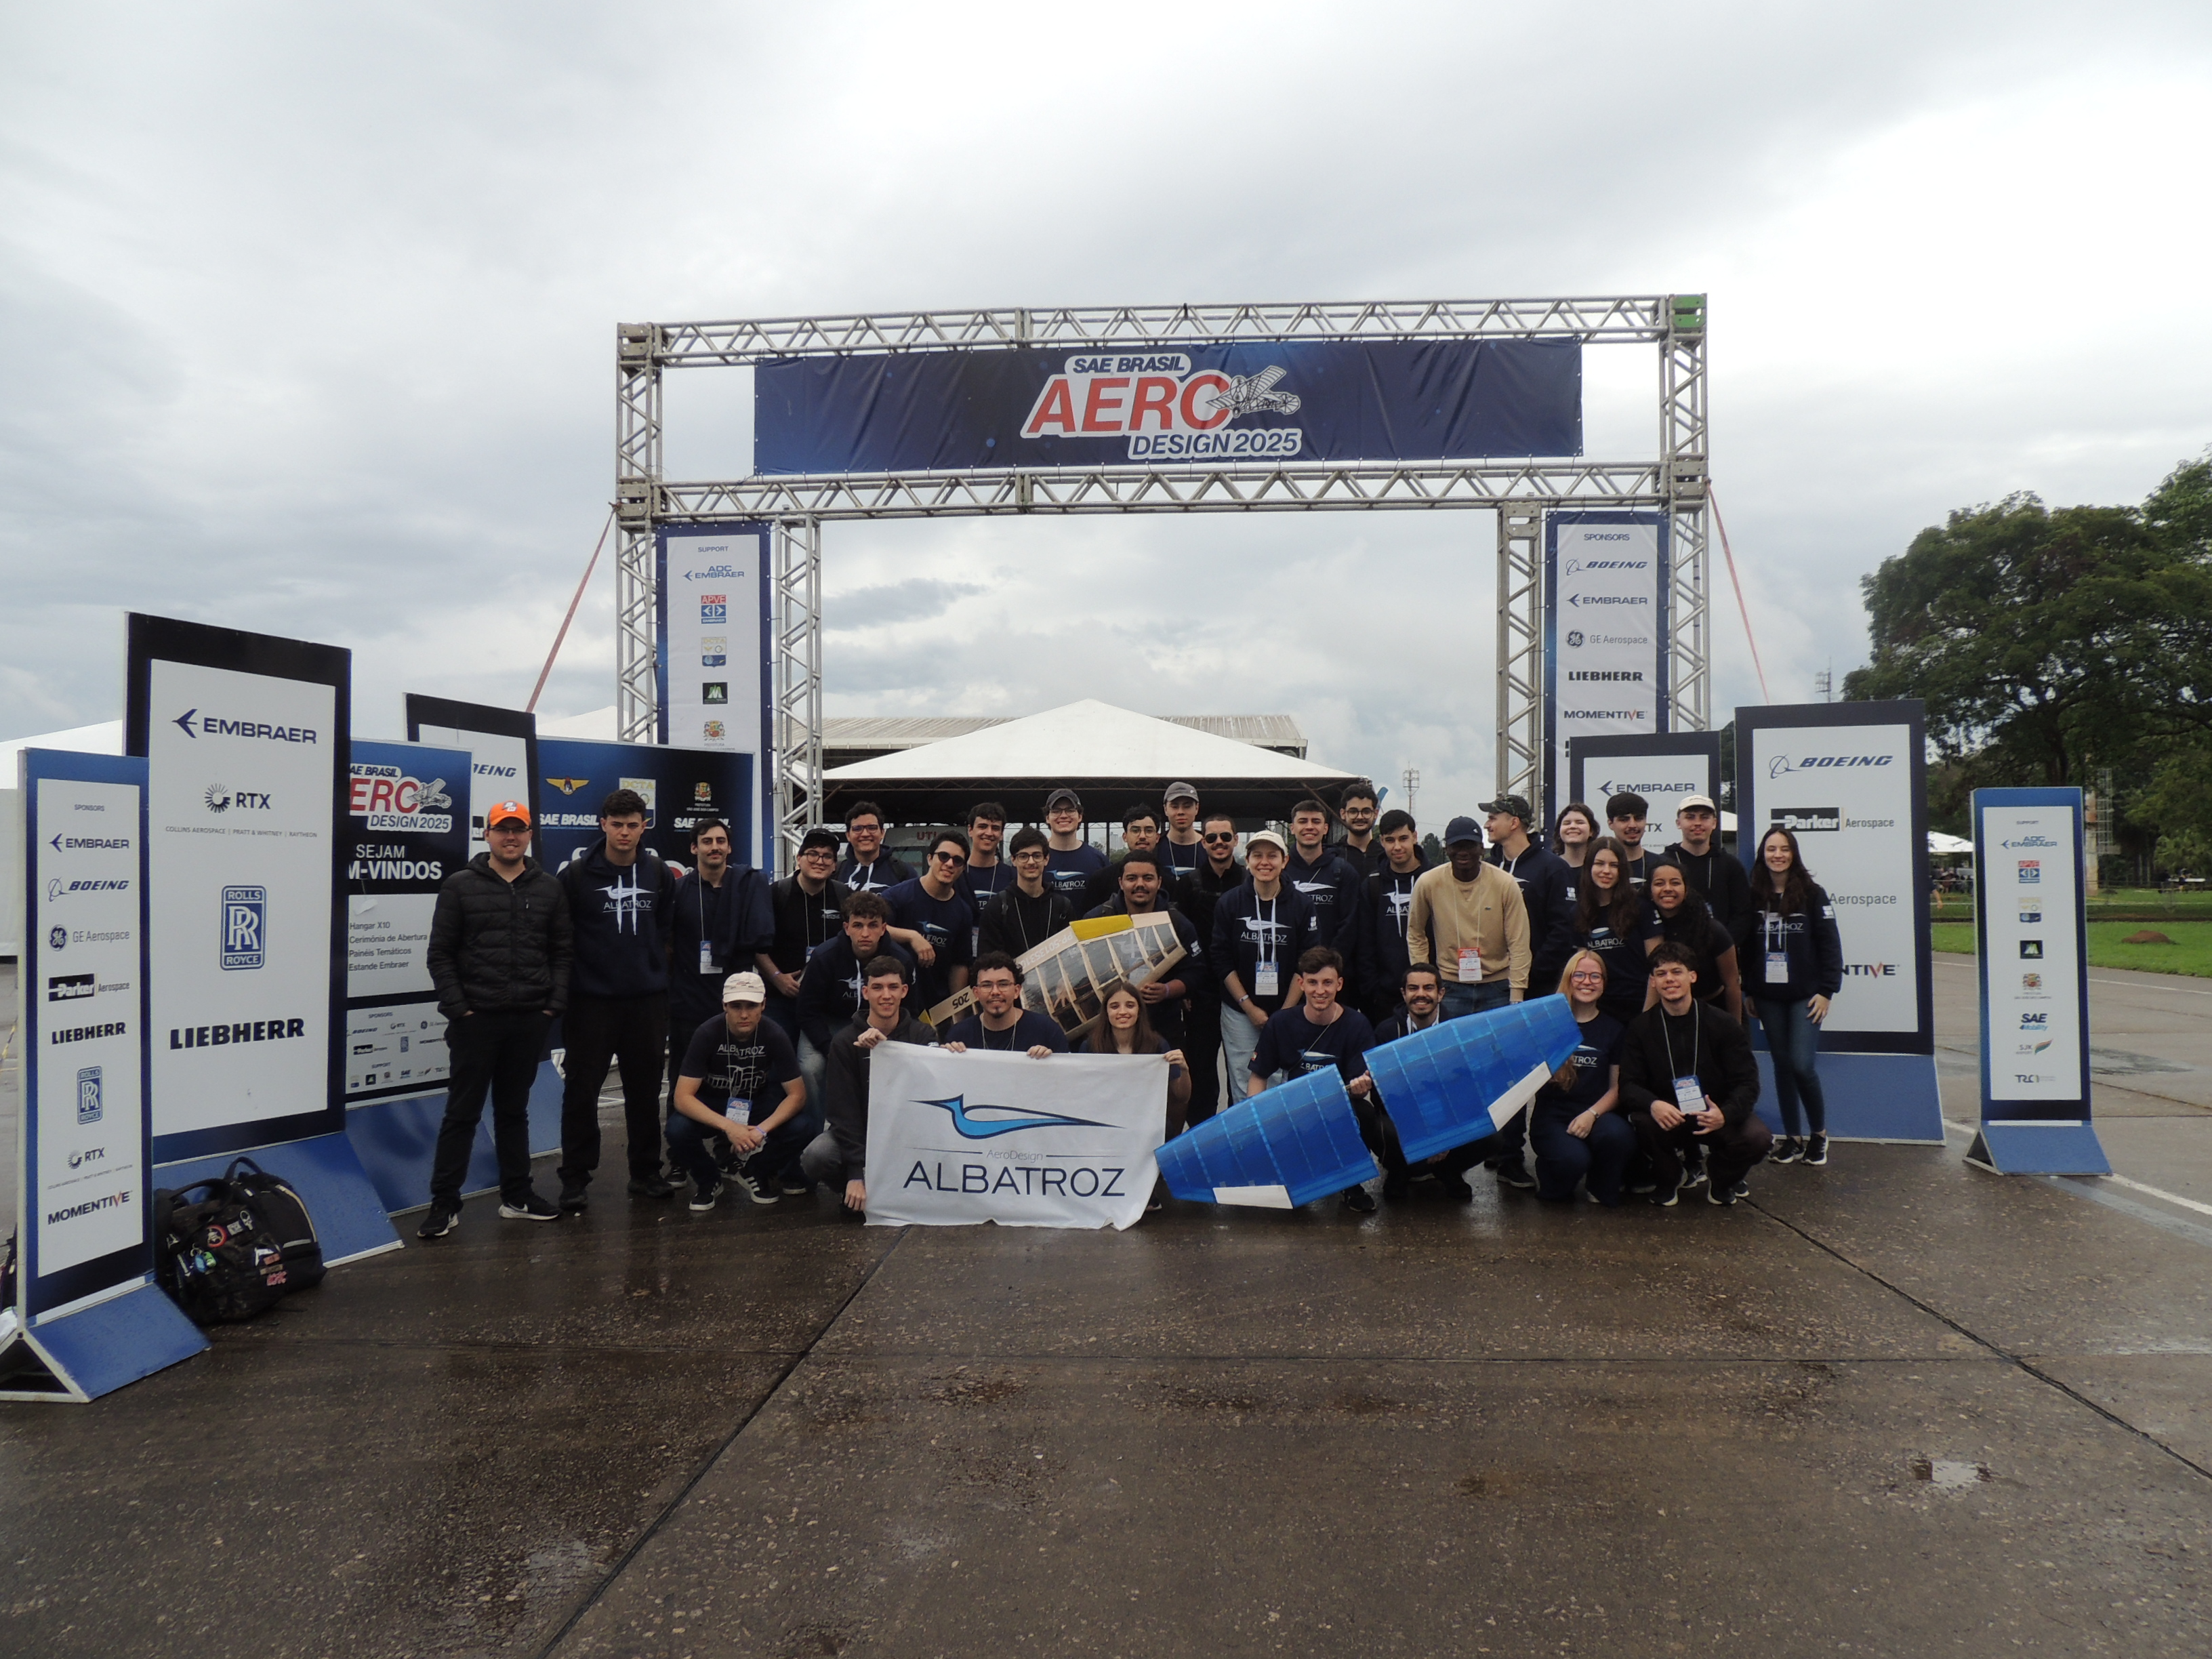
\includegraphics[width=0.5\linewidth]{Textuais/Imgs/Introducao/DSCN3474.JPG}
    \label{fig:EquipeAlbatroz2025_fotinho}
    \\ Fonte: Equipe Albatroz.
\end{figure}

O sistema motopropulsor constitui um subsistema crítico no projeto de aeronaves de competição, uma vez que seu desempenho determina diretamente a capacidade de carga útil da aeronave, fator decisivo nas competições da SAE \cite{SilvaGomes2022}. Neste contexto, os motores BLDC (\textit{Brushless Direct Current}) são empregados quase que universalmente. Sua adoção é impulsionada não apenas por vantagens técnicas intrínsecas — como alta eficiência e elevada densidade de potência \cite{Krishnan2017} — mas também por um requisito regulamentar: desde 2022, o regulamento da SAE Brasil Aerodesign restringe o uso a motores elétricos sem escovas, consolidando-os como a solução padrão para a categoria \cite{SAEBrasil2024}. 

Historicamente, a equipe Albatroz realizava medições de forma fragmentada, carecendo de um sistema integrado para aquisição sincronizada e abrangente de dados, o que limitava a profundidade e confiabilidade das análises de desempenho propulsivo, como pode ser visualizado na \autoref{fig:CMP_concepcao}.

\begin{figure}[ht]
    \centering
    \caption{Bancada de Ensaios de Desempenho}
    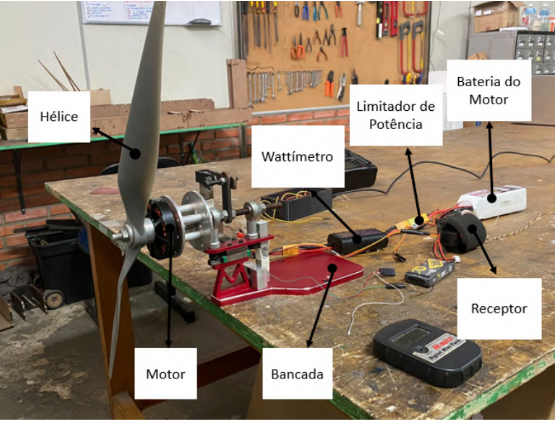
\includegraphics[width=0.5\linewidth]{Textuais/Imgs/Introducao/BancadaDesempenho.png}
    \label{fig:CMP_concepcao}
    \\ Fonte: \cite{albatroz2023desempenho}.
\end{figure}

Para diagnosticar e caracterizar esses motores, é comum recorrer a técnicas de estimação de estado, que permitem inferir variáveis internas não medidas diretamente. Em motores BLDC, o uso de técnicas como o método \textit{sensorless} é particularmente vantajoso, pois alia confiabilidade à redução de custos com sensores mecânicos adicionais \cite{Krishnan2017}.

Diante desse panorama, verifica-se uma lacuna técnica na infraestrutura de testes da equipe: a ausência de uma bancada de ensaios automatizada e instrumentada que possibilite a aquisição sincronizada de dados elétricos do motor, parâmetros aerodinâmicos da hélice e a validação dos algoritmos de estimação. Trabalhos anteriores em equipes similares desenvolveram bancadas focadas em medições de tração ou parâmetros elétricos de forma isolada (e.g., \cite{Costa2021}), mas frequentemente não integram uma arquitetura de aquisição unificada que correlacione diretamente os fenômenos elétricos, mecânicos e aerodinâmicos.

Portanto, a motivação central deste trabalho é o desenvolvimento de uma bancada de medição avançada para sistemas propulsivos com motores BLDC. A proposta avança além da simples automação, integrando: 1) um sistema de aquisição elétrica de alta precisão com \textit{hardware} dedicado; 2) a modelagem dinâmica do motor e o projeto de um observador de estados por modos deslizantes para estimação de velocidade e torque; 3) a integração dos sensores aerodinâmicos existentes; 4) uma infraestrutura de comunicação em rede robusta; e 5) um \textit{software} de supervisão. O objetivo final é fornecer uma ferramenta de caracterização que permita a aquisição sincronizada e o comparativo sistemático entre as grandezas medidas diretamente (tensão, corrente, tração) e as variáveis estimadas pelo observador (força eletromotriz, velocidade angular, torque no eixo).

Para atingir esse propósito, este trabalho estrutura-se nos objetivos específicos detalhados, os quais guiarão o desenvolvimento desde a concepção do \textit{hardware} e o projeto do observador até a implementação do sistema de comunicação e da interface de \textit{software}, culminando na validação experimental do conjunto.

\newpage
\section{Objetivos}

\subsection{Objetivos Gerais}

Desenvolver um sistema integrado de aquisição de dados adaptando a bancada atual de ensaios para conjuntos motopropulsores da equipe \textit{Albatroz Aerodesign}.

\subsection{Objetivos Específicos}
\begin{enumerate}
    \item \textbf{Projetar e implementar o sistema de medição do motor BLDC:}
    Projetar e fabricar uma placa de circuito impresso (PCB) para aquisição da
    tensão e da corrente nos terminais do motor BLDC, contemplando sensores de
    corrente por fase, circuitos de condicionamento de sinal e amostragem
    sincronizada da tensão de cada enrolamento, de modo a fornecer os dados
    necessários à modelagem e ao projeto do observador.

    \item \textbf{Modelar o motor BLDC e projetar o observador de estados:}
    Desenvolver o modelo matemático da dinâmica do motor BLDC, contemplando:
    \begin{itemize}
        \item a identificação experimental dos parâmetros elétricos e mecânicos
        (resistência de fase, indutância, constantes de torque e de força
        contraeletromotriz, momento de inércia e coeficiente de atrito viscoso);
        \item a formulação das equações de estado no referencial $\alpha\beta$
        que relacionam tensão aplicada, corrente e velocidade do rotor;
        \item o projeto e a implementação de um observador por modos deslizantes
        para a estimação em tempo real da força contraeletromotriz
        (\textit{back-EMF}), da velocidade angular e do torque no eixo, a partir
        das medições de corrente e tensão de fase.
    \end{itemize}

    \item \textbf{Implementar o sistema de medição aerodinâmica da hélice:}
    Integrar e condicionar os sinais dos sensores da bancada existente — tubo de
    Pitot e células de carga — para a medição simultânea de tração, momento e
    velocidade do escoamento, com transmissão dos dados em tempo real por um
    servidor de comunicação UDP embarcado.

    \item \textbf{Integrar os nós de aquisição e o supervisório em uma rede
    Ethernet:} Estabelecer a infraestrutura de comunicação com Protocolo de Controle de Transmissão e Protocolo de Datagrama do Usuário (TCP/UDP) que interliga
    as placas SIBA e SAME ao software de supervisão, definindo o protocolo de
    troca de pacotes e a estrutura de telemetria que padroniza os dados
    trafegados entre o \textit{firmware} embarcado e a aplicação \textit{desktop}.

    \item \textbf{Desenvolver o software de supervisão em Python:} Implementar
    uma aplicação para monitorar, comandar e parametrizar o conjunto
    motopropulsor, registrar os dados em formato padronizado \textit{Comma-Separated Values} (CSV) e sinalizar
    inconsistências em cada medição, comunicando-se com o sistema embarcado.
\end{enumerate}

\section{Estrutura do Trabalho}

Este trabalho está organizado em cinco capítulos, estruturados de forma a
conduzir o leitor desde a fundamentação teórica até a validação experimental
do sistema desenvolvido.

{Capítulo~\ref{cap:introducao}}: apresenta a contextualização e a
motivação do trabalho no âmbito do projeto Albatroz Aerodesign, delimitando a
lacuna técnica identificada na infraestrutura de ensaios da equipe, os
objetivos gerais e específicos e a própria estruturação do texto.

\textbf{Capítulo~\ref{cap:fundamentacao}}: reúne a fundamentação teórica
necessária ao desenvolvimento, abordando o princípio de funcionamento e a
modelagem do motor BLDC, o referencial estacionário $\alpha\beta$ de Clarke, o
Observador por Modos Deslizantes (SMO), a aerodinâmica de propulsores e a
instrumentação empregada na bancada, incluindo a infraestrutura de comunicação
e a arquitetura de gerenciamento de recursos no Zephyr.

\textbf{Capítulo~\ref{cap:metodologia}}: descreve os procedimentos e as
decisões de projeto adotados, detalhando a identificação experimental dos
parâmetros do motor, a parametrização do observador, a arquitetura de
\textit{firmware} das placas SIBA e SAME, a interface de supervisão e a
montagem mecânica e elétrica do conjunto.

\textbf{Capítulo~\ref{cap:resultados}}: apresenta e discute os resultados,
confrontando as grandezas medidas diretamente com as estimadas pelo
observador, e reportando a medição de parâmetros, o ajuste automático dos
ganhos do SMO e a identificação dos coeficientes aerodinâmicos.

\textbf{Capítulo~\ref{cap:conclusao}}: sintetiza as conclusões do trabalho e
apresenta as sugestões para trabalhos futuros.
